\documentclass{beamer}

\usepackage[utf8]{inputenc}
\usepackage{tikz}
\usepackage{hyperref}
\usepackage{listings}
\usepackage{float}
\usepackage{media9}

\graphicspath{{./images/}}
\addmediapath{./media/}

\usetheme{Madrid}

\title{The Legend of Link}

\author{David Antuña \and Jaime Bas \and Irene González \and José Luis Moreno}

\institute[UCM]
{
  DVI\\
  Universidad Complutense de Madrid
}

\date{Curso 2017-18}

\subject{Making a game with Quintus}

\pgfdeclareimage[height=0.5cm]{university-logo}{images_ignore/university-logo-filename}
\logo{\pgfuseimage{university-logo}}

\AtBeginSubsection[]
{
  \begin{frame}<beamer>{Contenidos}
    \tableofcontents[currentsection,currentsubsection]
  \end{frame}
}

\begin{document}

\begin{frame}
  \titlepage
\end{frame}

\begin{frame}{Contenidos}
  \tableofcontents
\end{frame}

% Section and subsections will appear in the presentation overview
% and table of contents.
\section{aiTrack}

\subsection{¿Qué es?}

\begin{frame}{¿Qué es?}
Es un nuevo componente para la libreria 2d que otorga a un sprite la capacidad
de localizar, seguir y atacar a otro(s).

\medskip

Está basado en cuadrídula, por lo que solo sirve para 2d con vista cenital.
\end{frame}

\subsection{Propiedades}

\begin{frame}{Propiedades}
\begin{itemize}
  \item \textit{view\_range} y \textit{attack\_range}: Rango al cual se activará
    el movimiento o ataque
  \item \textit{tile\_size}: Tamaño de un tile de la cuadrídula
  \item \textit{vfactor}: Multiplicador de velocidad\\
    v = tile\_size * vfactor
  \item \textit{attacking} y \textit{tracking}: Indica si el sprite está
    atacando o persiguiendo a un enemigo
  \item \textit{reloadSpeed}: Tiempo de enfriamiento de un ataque
  \item \textit{reload}: Enfriamiento actual
  \item \textit{track\_class}: Lista de clases con las que el sprite interactuará
\end{itemize}
\end{frame}

\subsection{Funcionamiento}

\begin{frame}{Funcionamiento}
En cada iteración del bucle de juego el modulo Scenes activará la señal
\textbf{range.check} para todos los componentes de la escena.

\medskip

El componente escucha esta señal y comprueba la distancia entre la entidad y
los elementos de la escena cuya clase esté en la lista.

\medskip

Hay tres posibilidades:
\begin{itemize}
  \item No está en rango $\rightarrow$ No ocurre nada
  \item Está en rango de ataque $\rightarrow$ Activa la señal
    \textbf{range.attack}
  \item Está en rango de movimiento $\rightarrow$ Activa la señal
    \textbf{range.view}
\end{itemize}
\end{frame}

\subsection{Triggers}

\begin{frame}{range.attack}
Esta señal activa la función attack del componente.

\medskip

Si reload es menor o igual que 0.
\begin{itemize}
  \item Activa el atributo attacking
  \item Resetea el tiempo de enfriamiento
  \item Invoca la función hit y le pasa el atributo damage de la entidad
\end{itemize}
\end{frame}

\begin{frame}{range.view}
Esta señal activa la función move del componente.

\medskip

Esta función trata de equiparar el componente x e y de la entidad a los del
elemento que esta siguiendo.

\begin{center}
  vx = $\pm$ tile\_size * vfactor\\
  vy = $\pm$ tile\_size * vfactor
\end{center}
\end{frame}

\subsection{Demostración}
\begin{frame}{Demostración}
  \centering
  \includemedia[
    activate=onclick,
    width=.5\textwidth
  ]{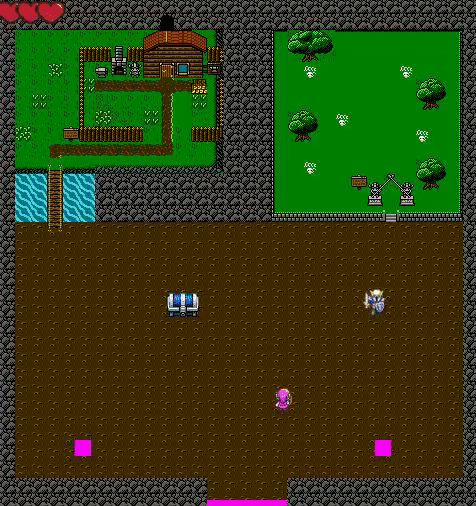
\includegraphics{Tracker-0.png}}{Tracker.mp4}
\end{frame}

\section{Componente stepControls}

\subsection{Problema}

\begin{frame}{Problema}
Para que el sprite se pueda mover en las 4 direcciones usamos el componente
de Quintus stepControls pero genera clipping al combinarse con nuestro aiTrack.

\medskip

El componente comprueba si la entidad colisiona y de hacerlo la devuelve al
origen, el problema es que los enemigos te persiguen y este componente impide
que el sprite escape.
\end{frame}

\begin{frame}{Código}
  \lstinputlisting{code/stepProblem.js}
\end{frame}

\subsection{Solución}

\begin{frame}{Problema}
Para solucionar este problema nos aprovechamos de un atributo de los
sprites en los que usamos este componente, todos tienen el atributo direction.

\medskip

Gracias a dicho atributo sabemos en que dirección se esta moviendo por lo que
podemos modificar el código para que se resetee la posicion solo si se mueve
hacia el objeto.
\end{frame}

\begin{frame}{Código}
  \lstinputlisting{code/stepSol.js}
\end{frame}

\end{document}
